%% $RCSfile: proj_report_outline.tex,v $
%% $Revision: 1.3 $
%% $Date: 2016/06/10 03:41:54 $
%% $Author: Mayur Panchal$

\documentclass[11pt
              , a4paper
              , twoside
              , openright
              ]{report}


\usepackage{float} % lets you have non-floating floats

\usepackage{url} % for typesetting urls

\usepackage{xspace} % space after trademarks specifically

\usepackage{pdfpages}

\let\OldTexttrademark\texttrademark
\renewcommand{\texttrademark}{\OldTexttrademark\xspace}%
\setlength{\parskip}{1em}

%
%  We don't want figures to float so we define
%
\newfloat{fig}{thp}{lof}[chapter]
\floatname{fig}{Figure}

%% These are standard LaTeX definitions for the document
%%                            
\title{Network switching fabric for Gigabit links}
\author{Mayur Panchal}

%% This file can be used for creating a wide range of reports
%%  across various Schools
%%
%% Set up some things, mostly for the front page, for your specific document
%
% Current options are:
% [ecs|msor|sms]          Which school you are in.
%                         (msor option retained for reproducing old data)
% [bschonscomp|mcompsci]  Which degree you are doing
%                          You can also specify any other degree by name
%                          (see below)
% [font|image]            Use a font or an image for the VUW logo
%                          The font option will only work on ECS systems
%
\usepackage[image,ecs]{vuwproject}

% You should specifiy your supervisor here with
%     \supervisor{Firstname Lastname}
% use \supervisors if there is more than one supervisor

\supervisors{Bryan Ng, Robin Dykstra}

% Unless you've used the bschonscomp or mcompsci
%  options above use
%   \otherdegree{OTHER DEGREE OR DIPLOMA NAME}
% here to specify degree

\otherdegree{Bachelor of Engineering with Honours in Electronic and Computer Systems Engineering}

% Comment this out if you want the date printed.
\date{}

\begin{document}

% Make the page numbering roman, until after the contents, etc.
\frontmatter

%%%%%%%%%%%%%%%%%%%%%%%%%%%%%%%%%%%%%%%%%%%%%%%%%%%%%%%

%%%%%%%%%%%%%%%%%%%%%%%%%%%%%%%%%%%%%%%%%%%%%%%%%%%%%%%

%\begin{abstract}

%A short description of the project goes here.

%\end{abstract}

%%%%%%%%%%%%%%%%%%%%%%%%%%%%%%%%%%%%%%%%%%%%%%%%%%%%%%%

\maketitle

%\chapter*{Acknowledgments}\label{C:ack} 
Any acknowledgments should go 
in here, between the title page and the table of contents.  The 
acknowledgments do not form a proper chapter, and so don't get a 
number or appear in the table of contents.

\tableofcontents

% we want a list of the figures we defined
\listof{fig}{Figures}

%%%%%%%%%%%%%%%%%%%%%%%%%%%%%%%%%%%%%%%%%%%%%%%%%%%%%%%

\mainmatter

%%%%%%%%%%%%%%%%%%%%%%%%%%%%%%%%%%%%%%%%%%%%%%%%%%%%%%%

% individual chapters included here
\chapter{Introduction}\label{C:intro}

\par Fast internet connections are becoming more and more desired as high bandwidth media consumption and internet 
based services grow in popularity. Speed of an internet connection can be separated into two distinct metrics, 
latency and bandwidth. Latency is the time taken for information to travel from one place to another and the delay 
introduced by the device itself, while bandwidth is the amount of information that can flow reliably from end to end.
When a user is accessing a website, such as Facebook, their requests traverse multiple network devices (physical 
hardware) to reach that website's servers. Throughout this travel, each network device introduces some latency, as 
there is processing time required to send information to the right destination. Although this delay is very small, 
over the course of multiple hops it can become significant. Measuring this small latency with current solutions is
convoluted and without the right systems, can be unreliable. By measuring this latency, we can enable research to
reduce latency to create a faster internet.

\section{Problem}

\par There has been research dedicated to reducing latency. Some ways to reduce this latency include making “smart” network routers \cite{smartrouters} and low latency wireless systems \cite{5g}. 
This research is reaching the point where network traffic can have latency as little as 1ms \cite{lessthan1ms} or below.
To advance further, new tools need to have the capability of measuring this latency.

\par Existing hardware solutions to measuring latency are capable of measuring less than 1 ms but require some 
additional training in the software suite provided with the hardware \cite{dagfeatures}. Additional processes attached
to hardware based methods can require dedicated computers for the measurement and analysis of networks. This means 
that each researcher would require an understanding of the software suite accompanied with a dedicated computer 
all setup for specific tests to be run. Each different test would require reconfiguring of both hardware and software.
This drives the cost of using the device up, in terms of both time and money.

\par Current software solutions can measure latency in ethernet network traffic down to a resolution of
milliseconds and sometimes microseconds \cite{pingisbad}. There are no software solutions that can measure
latency in the order of nanoseconds reliably \cite{timeinlinux}. Measuring the latency in nanoseconds is needed as
network switches have very low latency and the time between ingress and egress can range from
microseconds to nanoseconds. If it could be measured accurately, then analysis could be performed
on network traffic through network switches to research new ways to reduce latency.

\par Existing methods to measure latency within microseconds and nanoseconds require monolithic devices which need 
setting up and installing device drivers, proprietary software, or even a replacement of existing hardware systems.
Once setup, these devices often require data conversion of results to be compatible with data analysis methods and 
evaluation programs. Occasionally these programs are embedded within in manufacturers software, but the user is 
limited to what the manufacturer has chosen as relevant outputs for the user. These can be useful most of the time, 
but occassionally the user would need to export the data to another data analysis tool they are familiar with for 
futher processing. This inflexibility is prominent in many high end network performance analysis tools, causing 
delays in retrieving test results for evaluation.

\par A reduction in network latency would be a huge boon to future technologies. For example, less
latency in video streaming can enable doctors from remote locations to perform surgery with
minimal lag between actions and responses \cite{remotesurgery}. The stock market is another example of improvement with
this technology, as less latency ensures that stock market trade deals can be completed faster.

\begin{quote}
    \centering
    ``We are running through the United States with dynamite and rock saws, so that an algorithm can
    run three microseconds faster.`` \em --- Kevin Slavin, How Algorithms shape our world \cite{tedTalkAlgorithms}
\end{quote} 

\par Many improvements made at a nanosecond scale can add up to microseconds or even milliseconds of latency
reduction. Improvements cannot be done without knowing how much this can improve by without the tools to measure it.

\par A software based approach has the limitation that the timing functions must be processed by a
Central Processing Unit (CPU) \cite{CPUtiming}. This means the counters for timing functions could be offset from the true value. Higher
resolution latency measurements can be achieved through a hardware implementation of a packet
timer. This circumvents the limitations of a software based approach.

\section{Solution}

Latency occurs the instant that a network packet is sent from a computer. The processing times for the network packet
to flow through the networking stack in the operating system can be considered a constant unavoidable delay which is
not in the scope of this project.

Because the nature of when the latency occurs, it would be best measured by considering the raw electronic signals 
from the ethernet port on the device to ensure there is no operating system lag. To achieve this, microcontrollers, 
discrete logic gates and a Field Programmable Gate Array could be implemented. A microcontroller could be used but 
then the same issues arise, that a CPU clocking through instructions would deviate the true timing counter value. 
Another approach would be to use discrete logic gates to measure the timing accurately, but this will become 
complicated very rapidly, and propagation delays through discrete devices would reduce the accuracy. Hence the 
preferred choice is to implement the packet latency measurement unit on a Field Programmable Gate Array (FPGA). More 
information about FPGA’s is in the Background section of the report. This way complex digital designs can be 
simplified down to a simple set of blocks, and there is no overhead that a processor would introduce. The drawback 
to using an FPGA is that the learning curve to developing on the platform is quite steep, and also communication 
with existing systems is difficult and is usually aided by the use of a microcontroller (such as an ARM or x86 based 
co-processor)

\par This report will focus on the work done so far in implementing a FPGA based packet latency timing
device. This project is limited to Ethernet based networks as they are most widely used \cite{etherneteverywhere}.

\chapter{Background}\label{C:back}

\section{Network packet}

\par Communication between computers is established through the means of physical connections and protcols overlaying on top of this. 
A widespread communication protocol is to break down each point of communication into discrete pieces called network packets.
These network packets contain many layers (Figure: \ref{fig:OSIModel}) of communication information.
Communication layers can be broken down into a few independent layers which hold specific purposes. 
Each layer contains information which can aid with transporting the information to the correct computer securely.
As each layer is independent, each higher layer does not affect the forthcoming layers.
High layers of the model are for purposes such as reliability of data and the data itself in the packet.
For the purposes of this project, an explanation of only the first three layers of the Open Systems Interconnection (OSI) model is concerned.

\begin{figure}[H]
    \begin{center}
        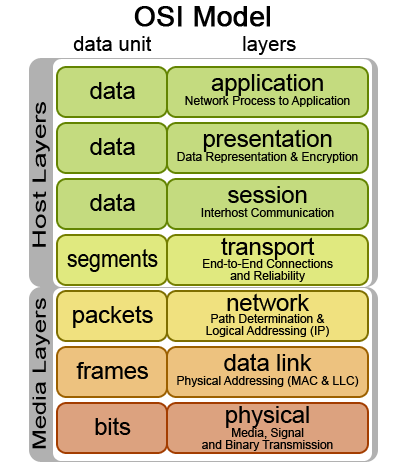
\includegraphics[width=5cm,height=5cm,keepaspectratio]{Images/OSIModel.png}
        \caption{OSI Model}
        \label{fig:OSIModel}
    \end{center}
\end{figure}

\subsection{Layer 1: Physical}

\par The physical layer is specifying the electrical and physical medium that is used to transport individual bits from one computer to another.
Two or more computers can be connected through many different physical mediums such as copper wiring and light fibers. 
Each medium has specific pros and cons, from implementation costs to throughtput capabilities.
The physical layer is responsible for transmitting and receiveing unstructured data.
Communication can be either Simplex, Half Duplex or Full Duplex.
The network topology is defined by how the physical layer is configured.
An example of a phyiscal medium is a copper medium is used to link two devices together.
This project will be investigating the latency present in a Gigabit Ethernet system, using copper based medium.

\subsection{Layer 2: Data link}

Data link layer is responsible for node-to-node data communication. 
It links from one device to another, determing the connection status of two physically connected devices.
A feature of this layer, is the ability to detect and correct errors created at the physical layer.
The IEEE Standard 802 \cite{IEEE802} details how this layer is split into two sub layers, Media Access Control (MAC), and Logical Link Control (LLC).
This project will cover networking switches which distinguish different destination devices by their unique MAC addresses.

\subsection{Layer 3: Network}

Network layer provides functionality when sending data across a network.
End-to-end communication is aided by assigning each node in the network an address, which it identifies itself with.
This allows data to be passed through intermediate nodes, which would continue to traverse until the target node has been reached.
This project will not be including this layer, or any others higher than this, as the latency measurements involved are short, single node-to-node distances.

\section{Network Latency}

\subsection{Connection Time}

\subsection{Round Trip Time}

\section{Current Timing Solutions}

Timing of network packets can currently done through very expensive and bulky devices. 
For this reason, there are many software implementations that allow high speed packet processing.
The following software implementations have some restrictions on what hardware they can run on.
The precision to measure the latency of packets is unknown and needs to be investigated.
This project is to combine the flexibility of software and hardware to create a packet latency measurement utility.

\subsection{Data Plane Development Kit (DPDK)}

Data Plane Development Kit (DPDK) is a set of C libraries to allow for rapid processing of network packets.
It utilizes a few low level Application Programming Interfaces (APIs) to minimize the overhead of using a specific architecture computer.
Reducing this overhead of the CPU reduces the amount of latecy present in the act of measuring the time between packets itself.
This is a very good software solution to what is currently on the market, but one caveat to using this technology is that only specific hardware can be used.
The Network Interface Card (NIC) on the computer has to be compatible with the software.

\subsection{PF\textunderscore RING}

PF\textunderscore RING by ntop\texttrademark is a software solution for rapid network packet processing.
It is a network socket technology which improves the speed at which packets are captured by the processor.
Faster packet processing ensures that the time stamp placed on an ingress packet is accurate as it can be.
This is a software solution which could potentially work well, but is limited by the software latency of needing to be processed by a processor.
The NIC on the computer does not have to be a specific model, meaning this is a much more flexible solution.

\section{Measurement Techniques}

\subsection{Cut-Through}

\subsection{Store-and-Forward}

\section{Field Programmable Gate Array}

\subsection{Reconfigurable Macro Cells}

\subsection{FPGA vs Microcontroller}

\chapter{Design}\label{C:design}

\vspace{-3mm}

\begin{figure}[H]
    \begin{center}
        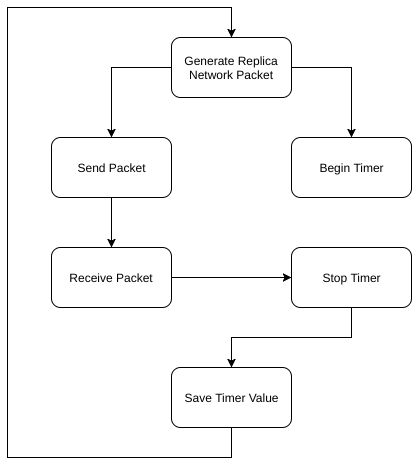
\includegraphics[keepaspectratio,width=8cm]{Images/MeasurementSequence}
        \caption{High-level flow chart of Measurement Sequence}
        \label{fig:measurementsequence}
    \end{center}
\end{figure}


The goal of this project is to create a device which can measure latency between two connections with high precision
and accuracy. Figure \ref{fig:measurementsequence} shows the high-level overview of what the device needs to be able 
to do. The following is the design decisions made to achieve the goal.

\section{Hardware Design}

For a platform to be flexible, it must be able to interact with any type of software and analysis tools. This is 
easily done by storing the data in an easy to use format (such as CSV) and providing it on a medium which is 
easily accessible and compatible with existing computers, which are typically x86 based PCs. Therefore, the choice 
was made to write the data to an SD card, which can be removed and inserted into a computer for post-processing, 
allowing the platform to be flexible. 

At the same time as being a flexible platform, the device needs to be able to measure low-level electrical signals 
with high reliability, while performing complex high-level instructions such as measuring the time between two 
signals. The best way to perform high precision actions with complex digital logic is a FPGA. The high-speed clocks 
involved with very precise timing instruments are too fast for a typical microcontroller or processor. 

A platform that combines both flexibility and ability to measure low level electrical signals is the Zynq line of 
FPGAs by Xilinx. These combine both an FPGA with an ARM processor, to allow for a full operating system to be run in 
tandem with operations on the FPGA.  The ARM processor can allow for future extensions onto the device to allow for 
interconnectivity with different kinds of storage mediums and even connect to the internet too, making it a highly 
flexible platform. 

An FPGA System block must generate a network packet that can be used to measure the latency. On an x86 based computer, 
this is done through the CPU, and an element called a MAC. The MAC is used to convert logic link control signals 
into physical hardware signals for the Ethernet Phy to interpret. An Ethernet Phy is required as the 802.3ab 
standard defines the electrical connection from one node to another to consist of 4 twisted pairs and the 
differential electrical signals required for this cable is not possible in an FPGA, or in a CPU, hence this is 
offloaded to an external IC. Connections consist of commonly found Category 5e and 6 cabling, which adheres to the 
tolerance for how many twists are performed per meter cable (Important for signal integrity). The connection between 
the MAC and the Ethernet PHY is performed through a hardware protocol standard called Media Independent Interface 
(MII) and then converted to the differential signals across the Category 5e/6 cable. The gigabit version of ethernet 
uses an extended version of MII called Reduced Gigabit Media Independent Interface (RGMII).

\section{Block Design (Concept)}

\vspace{-3mm}

\begin{figure}[H]
    \begin{center}
        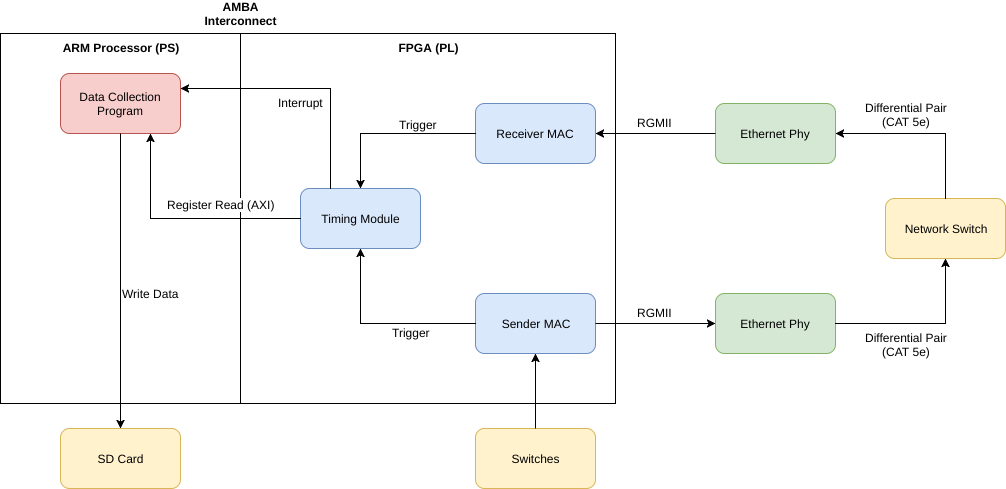
\includegraphics[keepaspectratio,width=15cm]{Images/BlockDesignConcept}
        \caption{Generic Block Design Concept. Blue represent FPGA logic blocks, Red represents Bare-Metal programs run on the ARM Processor, Green represents external ICs and Yellow represent other hardware external to the FPGA development board.}
        \label{fig:blockdesignconcept}
    \end{center}
\end{figure}

\vspace{-3mm}

\par The Sender MAC, the FPGA produces a repeated signal of a network packets and an interrupt to a timing module to 
begin counting. The number of packets per second (PPS) is controlled by hardware switches found on the development 
board itself. The Ethernet Phy converts these RGMII signals into differential signals what are used in communicating 
over CAT 5e/6 cable. This is then switched to the other Ethernet Phy, and the receiving end detects the incoming 
packet. The Receiver MAC detects the network packet, and produces an interrupt for the timing module to stop counting.

\par The Timing Module captures the events produced by the MACs and once a value is stored in the register, it 
produces an interrupt for the ARM Processor to begin reading the register. 

\par A program running on the ARM Processor intercepts the interrupt, and an interrupt service routine begins. This 
retrieves the value in the register and saves it to the SD card. Every time the interrupt is triggered, the value is 
appended to the end of a file stored on the SD Card. 

\section{Block Design (Implementation)}

\begin{figure}[H]
    \begin{center}
        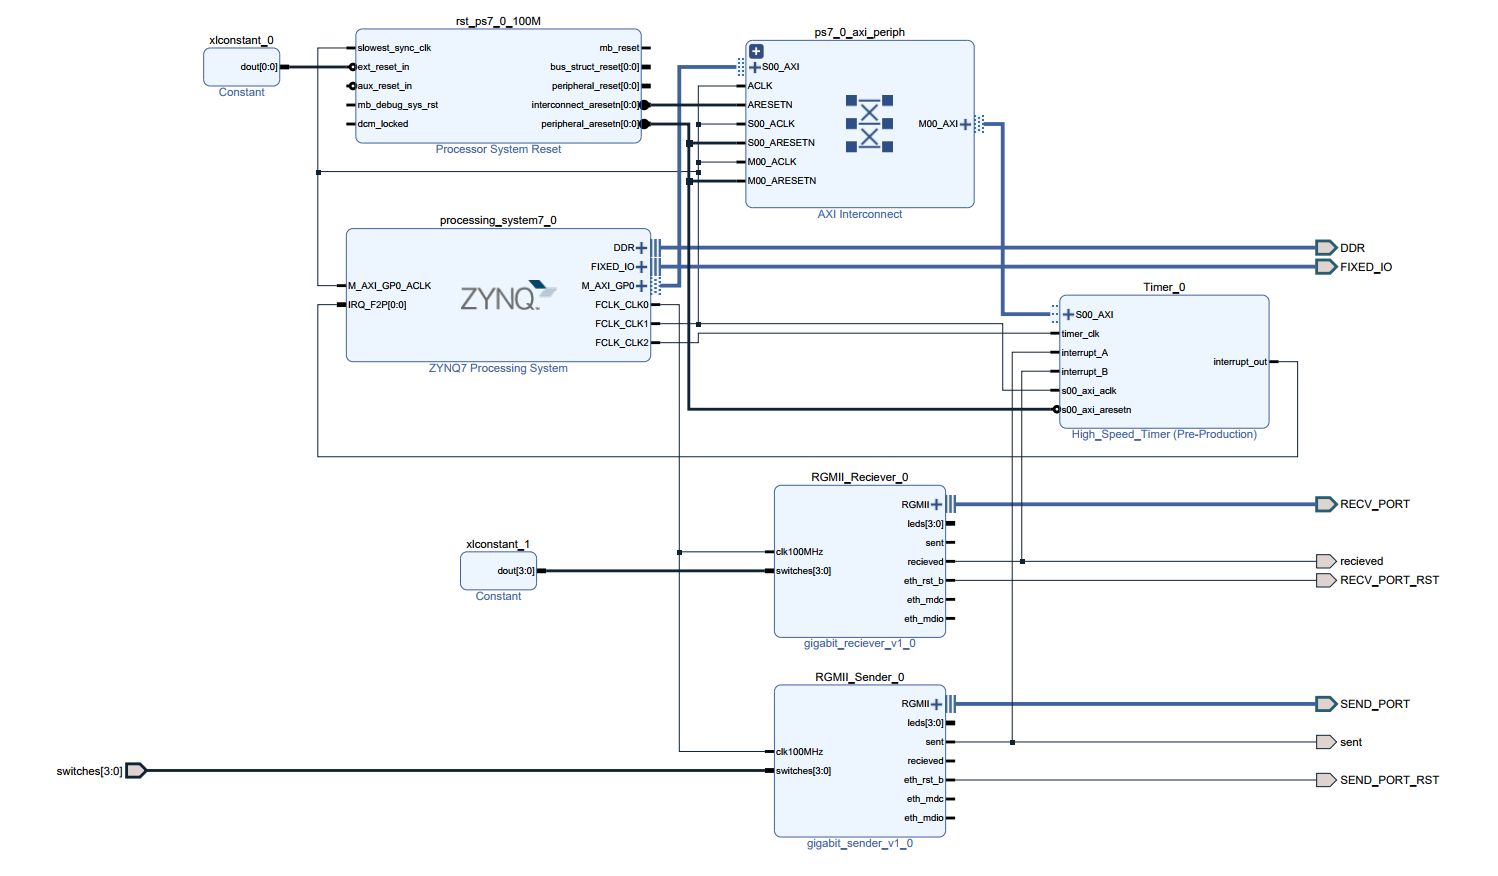
\includegraphics[keepaspectratio,width=15cm]{Images/BlockDesignImpl}
        \caption{FPGA Block Design Implementation. Each block is a VHDL module with the Input and Output exposed as 
        ports on the block itself.}
        \label{fig:blockdesignimpl}
    \end{center}
\end{figure}

\par Figure \ref{fig:blockdesignimpl} above shows the overall diagram of the FPGA logic blocks. This is the view 
through the IP integrator in Vivado 2017.2. Thicker lines in the diagram represent busses, while the thinner black 
lines represent single wires.  Connections on the left and right of the diagram represent Inputs and Outputs to the 
FPGA respectively. 

\par The extra blocks in the upper area of the diagram represent constructs needed for AXI peripherals. This allows 
the Processing Systen (PS) to interact and access registers found in the Programmable Logic (PL) of the FPGA. AXI manages the control signalling for buffering 
and clocking data in and out of the PS.

\section{Reduced Gigabit Media Independent Interface (RGMII)}

\par GMII is a full duplex interface between the MAC and an Ethernet Phy. As shown in Figure \ref{fig:gmiiwiring}, the physical wiring 
consists of 22 wires between the two devices. The signalling shown in Figure \ref{fig:gmiisignals} gives an example of how data is 
transferred to and from the Phy. Bytes transmitted to the Ethernet Phy are then converted and sent across the 
Cat5e/6 cable. RGMII is a Dual Data Rate Extension to GMII, by which the data is clocked on both the rising and 
falling edge of the clock. This means that one byte can be transmitted over four wires instead of 8, while keeping 
the same clock frequency. This is advantageous as there is commonly limited space on a PCB for wiring interconnects 
together, especially when there are more than 400 pins on a device (The XC7Z020-CLG484 has 
484 package pins). 


\chapter{Implementation}\label{C:impl}

\lstinputlisting[language=VHDL, firstline=36, lastline=37, basicstyle=\small]{Code/byte\string_data.vhd}

\lstinputlisting[language=VHDL, firstline=46, lastline=52, basicstyle=\small]{Code/edge\string_detector.vhd}

\lstinputlisting[language=VHDL, firstline=57, lastline=70, basicstyle=\small]{Code/InterruptTimer.vhd}

\lstinputlisting[language=VHDL, firstline=86, lastline=92, basicstyle=\small]{Code/packet\string_timer.c}

\chapter{Evaluation}\label{C:eval}

\section{Accuracy Testing}
\par To test the accuracy of the device, a loopback test was performed with different length of cables. This was 
setup so that there was no switch between two ethernet measurement ports, only an ethernet cable. The test is to 
ensure that the device is measuring the latency correctly, and able to detect the latency present in a specific 
length of cable. Latency measured from the device can be compared with the theoretical value of the latency which 
can be calculated using the following formula:

\[Latency = \frac{L}{cV_f}\]

\par Where L is the length of the cable, c is the speed of light (299,792,458 m/s) and V\textsubscript{f} is 
velocity factor of ethernet cables (0.65). 

\par A very short cable (4 cm) was used to measure the processing time, a constant added to every measurement. 
This processing time is the result of both Ethernet Phy’s converting between the two protocols (Differential Pairs 
and RGMII). Performing measurements with the short cable produced a mean value of 440 ns where 0.2095 ns of the 
measurement is attributed to the delay present in the cable.

\par This processing time is then removed from subsequent tests, making the latency values produced by the device 
purely the latency present in the cable. The goal from the tests is to ensure that the device is accurate to within
4 ns, which is the smallest interval of time that can be measured.

\par Tests were done with cables spanning 2 m, 3 m and 25 m long. These provided enough of a delay to measure with the
device, and enough data to characterise the accuracy of what cables are used. The measured value was plotted with 
the theoretical values of what delay would be present in the cable. To obtain the delay measurement, the test was 
run for 20 seconds on the device, with a packet transmission frequency of 500 packets per second. The mean value
of all packet latency measurements for that cable were then plotted versus the length of the cable.

\begin{figure}[H]
    \begin{center}
        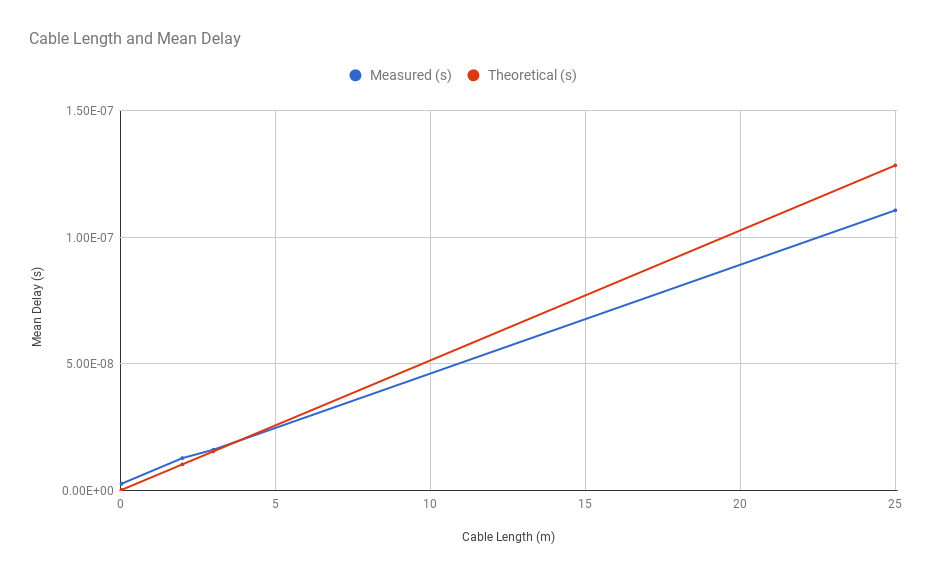
\includegraphics[keepaspectratio,width=15cm]{Images/CableTesting}
        \caption{Results from Accuracy Measurements}
        \label{fig:accuracyMeasurements}
    \end{center}
\end{figure}

\par As shown in ~\ref{fig:accuracyMeasurements}, the results from the device show a linear trend in latency due to 
length of the cable. The gradient difference of the theoretical line can be attributed to the fluctuation in 
velocity factor through the different cables.

\par The difference between the theoretical and measured value of the 25 m cable was 14 ns. This is not within the 
accuracy margin which was required, hence 2 m and 3 m cables are used for the reliablity tests as the difference was below 2 ns.

\section{Reliability Testing}

\par To test reliability of the device, repeated tests were performed to show that results would stay consistent
from test to test. As the goal of the project was to measure the latency in network swtiches, these tests were to 
measure the latency through a network switch and provide repeatable results. These results did not neccessarily have
to be accurate, as the accuracy was determined in the test in accuracy testing, hence these results are only to 
measure the reliability.

\par Results from the tests were compared to an existing DPDK software based latency measurement method. This was 
run on two separate machines which had clocks synchronoised using PTP protocol and as a result, the timings varied 
significantly. This comparision was to show that the software based methods have flexibility that hardware methods
are missing while also performing unreliably. The DPDK based system was compared to the FPGA based device by producing
a packet on one machine, then sending the packet through the network switch to arrive at the other machine, and the
time delta is returned from both machines. The FPGA device also performed the same task with the same cables, but 
the two connections arrived at the same machine.

\begin{figure}[H]
    \begin{center}
        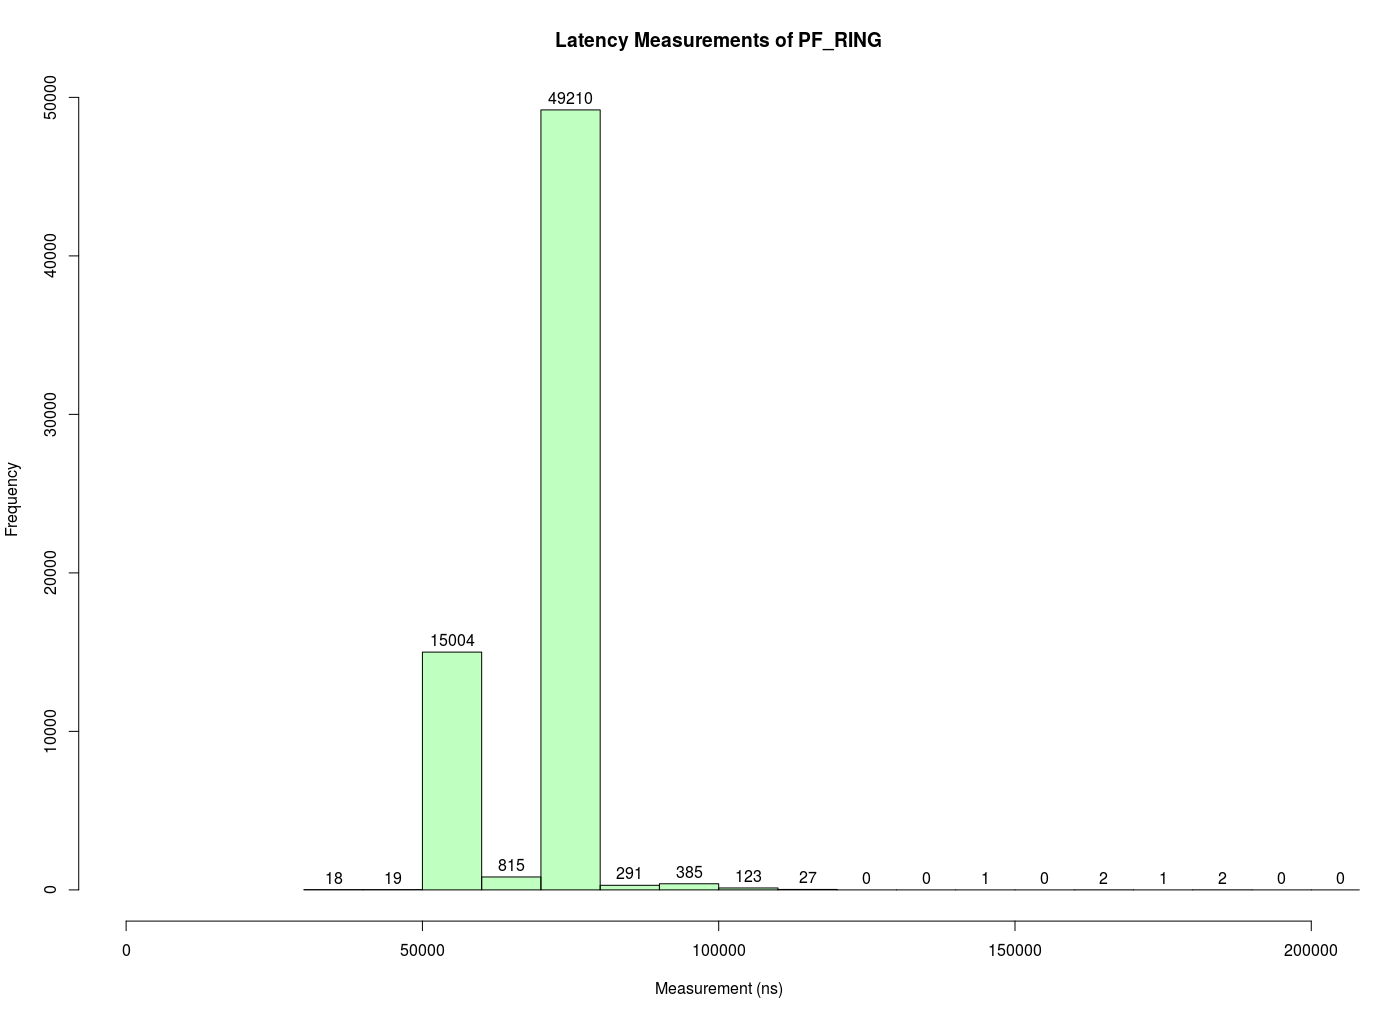
\includegraphics[keepaspectratio,height=7.5cm]{Images/pf_ring}
        \caption{Results from DPDK Reliability Measurements}
        \label{fig:DPDKReliability}
    \end{center}
\end{figure}

\begin{figure}[H]
    \begin{center}
        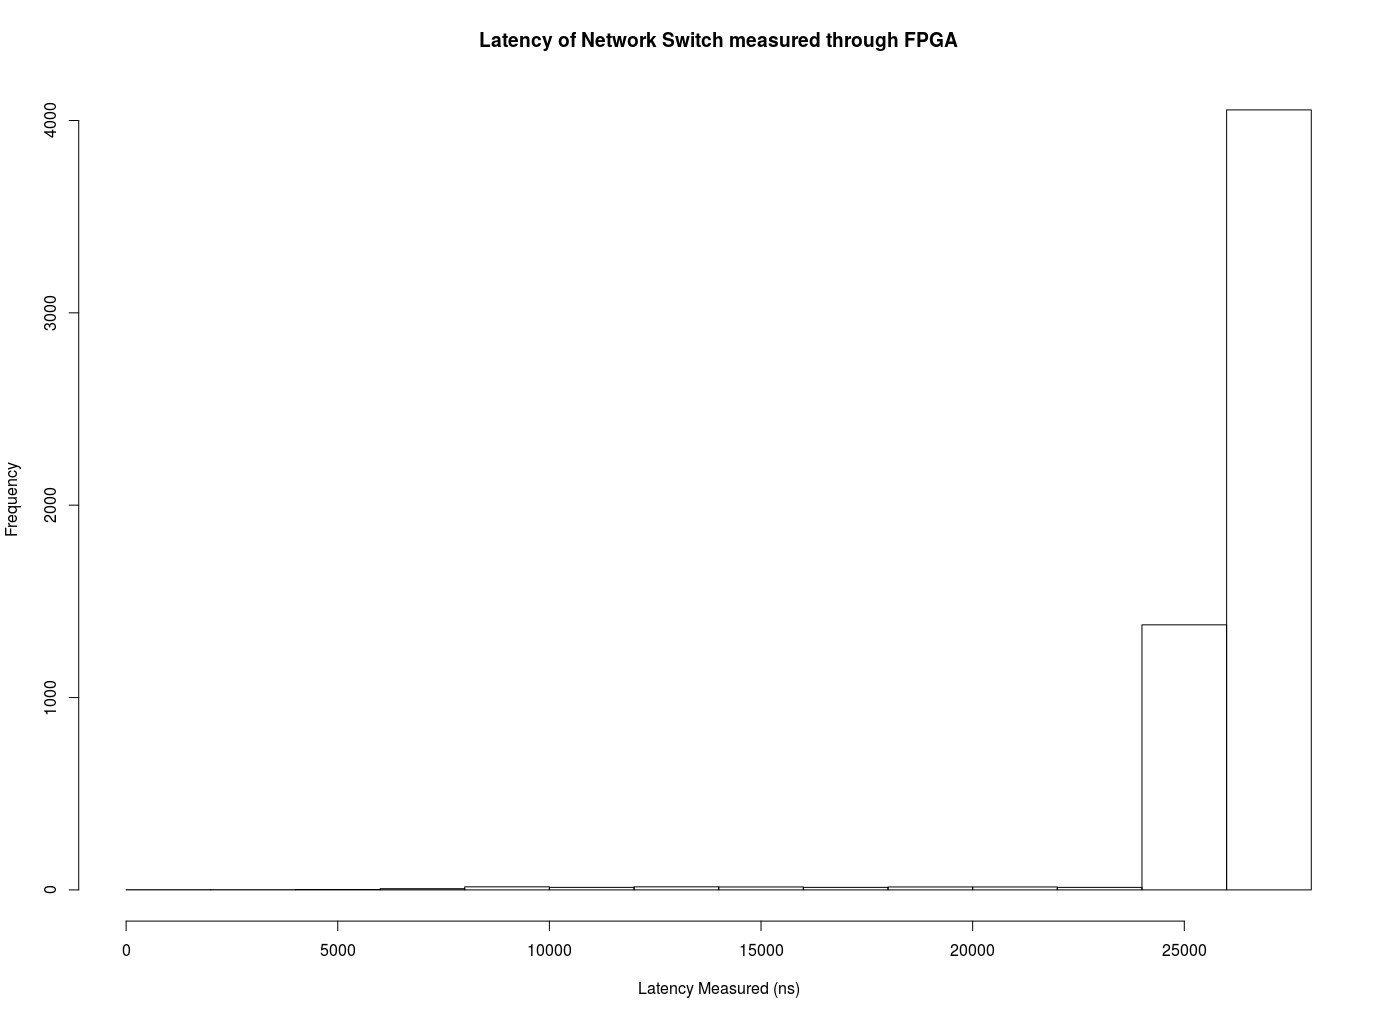
\includegraphics[keepaspectratio,height=7.5cm]{Images/TestPlot}
        \caption{Results from FPGA device Reliability Measurements}
        \label{fig:Test2Plot}
    \end{center}
\end{figure}

\par As seen in the results, the FPGA device produced a value lower than the mean value. This is very interesting, as
it is an unexpected result. Lower values produced by the device could be attributed to the device misinterpreting 
the reception of a previous test as the end of the current test. Regardless of this result, the device produced over 
10 times lower standard deviation compared with the results from the DPDK test setup. This can be concluded as a 
successful test.


%%%%%%%%%%%%%%%%%%%%%%%%%%%%%%%%%%%%%%%%%%%%%%%%%%%%%%%

\backmatter

%%%%%%%%%%%%%%%%%%%%%%%%%%%%%%%%%%%%%%%%%%%%%%%%%%%%%%%


%\bibliographystyle{ieeetr}
\bibliography{references}{}
\bibliographystyle{ieeetr}

\chapter{Appendix}\label{C:appendix}
\section{\\GitHub Link to Work}
https://github.com/Maeur1/ENGR489


\end{document}
